\begin{frame}{Formas de onda transitórias registradas}
  \small
  \begin{columns}[T,onlytextwidth]
    \begin{column}{0.48\textwidth}
      \centering
      \textbf{Registro com resposta monótona}

      \vspace{0.12cm}
      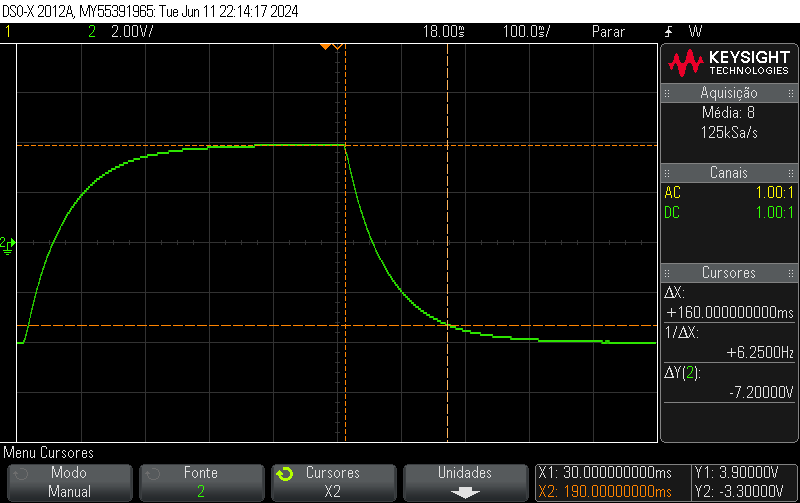
\includegraphics[width=\linewidth,height=0.43\textheight,keepaspectratio]{slides/img/transitorio_monotono.jpg}

      \vspace{0.12cm}
      Cursor em $-7{,}2\,\mathrm{V}$ e $160\,\mathrm{ms}$.\\
      Circuito 1: níveis de $-0{,}8\,\mathrm{V}$ (10\%) e $-7{,}2\,\mathrm{V}$ (90\%).
    \end{column}
    \begin{column}{0.48\textwidth}
      \centering
      \textbf{Registro com oscilação amortecida}

      \vspace{0.12cm}
      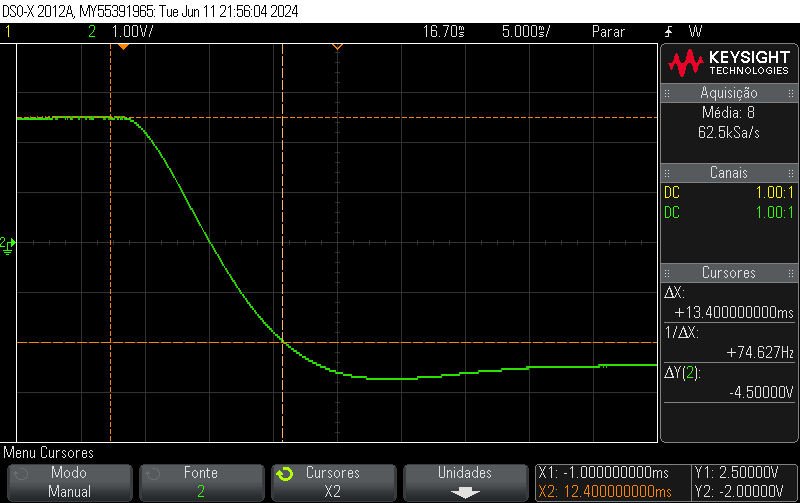
\includegraphics[width=\linewidth,height=0.43\textheight,keepaspectratio]{slides/img/transitorio_oscilatorio.jpg}

      \vspace{0.12cm}
      Cursor em $-4{,}5\,\mathrm{V}$ e $13{,}4\,\mathrm{ms}$.\\
      Circuito 2: níveis de $-0{,}5\,\mathrm{V}$ (10\%) e $-4{,}5\,\mathrm{V}$ (90\%).
    \end{column}
  \end{columns}

  \vspace{0.20cm}
  \centering\scriptsize
  Capturas transitórias preservadas. Os valores finais são $-8\,\mathrm{V}$ no circuito 1
  e $-5\,\mathrm{V}$ no circuito 2; os cursores mostram os registros das imagens.
\end{frame}
